\documentclass[notes]{subfiles}
\begin{document}
	\addcontentsline{toc}{section}{2.2 - Measures of Change at a Point - Graphical}
	\refstepcounter{section}
	\fancyhead[RO,LE]{\bfseries  \nameref{cs22}} 
	\fancyhead[LO,RE]{\bfseries \small \currentname}
	\fancyfoot[C]{{}}
	\fancyfoot[RO,LE]{\large \thepage}	%Footer on Right \thepage is pagenumber
	\fancyfoot[LO,RE]{\large Chapter 2.2}


\section*{Measures of Change at a Point - Graphical}\label{cs22}
	\subsection*{Tangent Lines and Secant Lines}
		\begin{defn}[Secant Line]
			Let $f$ be continuous and smooth function on the some input interval $[a,b]$.  Let $x_1 < x_2$ be two points in $[a,b]$.  The \textbf{secant line} through $x_1$ and $x_2$ is the line whose slope is \showto{ins}{\fbox{$\dfrac{f(x_2)-f(x_1)}{x_2-x_1}$}}\showto{st}{\\$ $ \\}
		\end{defn}
			
		The characteristic of a secant line is that it ``intentionally'' goes through $f$ in two points.  
		
		\begin{question}
			The formula for the slope of a secant line should look familiar; what's the other name we used for this?
		\end{question}
			\vs{.5}
			
		\begin{ex}
			Let $f(x) = x^2$.  Find the secant line through $x_1 = -\dfrac{1}{2}$ and $x_2 = 2$, then sketch $f(x)$ and the secant line.  
		\end{ex}
			\vs{3}
			
	\subsection*{Average Change vs. Instantaneous Change}
		Secant lines are drawn between two points on a graph.  As the distance between the points decreases, we get values of the independent axis which are closer and closer together; we can use a limiting process to find slope of the line through \emph{a single point}.  This is the called the \emph{tangent} line to the point.
			\vspace{.1in}
			
		\begin{defn}[Rate of Change]
			For smooth, continuous function $f$, the \textbf{rate of change} of the function at a particular point \showto{st}{\\[15pt]} $x_0$ is given by \showto{ins}{\fbox{the slope of the tangent line to the graph of $f$}}\showto{st}{\blank{2.5}}; the rate of change of $f$ at point $x_0$ is \showto{st}{\\[15pt]} denoted \showto{ins}{\fbox{$f'(x_0)$}}\showto{st}{\blank{1.5}}.
		\end{defn}
			\newpage
			
		\begin{defn}[Instantaneous ROC] 
			The \textbf{instantaneous rate of change} of a function $f$ measures \showto{ins}{\fbox{slope of the graph}\\ \fbox{of a function at a single point}}\showto{st}{\blank{2}\\[15pt] \blank{3}}.
		\end{defn}
			\vspace{.1in}
			
		\begin{ex}
			Estimate the slope of the tangent line to the curve $f(x) = x^2$ at $x = -\dfrac{1}{2}$ by drawing successive secant lines and computing the slope.
		\end{ex}
			\vs{2}
			
		\begin{ex}
			For the curve below, use successive secant lines to estimate $f'(0.4)$.
			\begin{flushleft}
				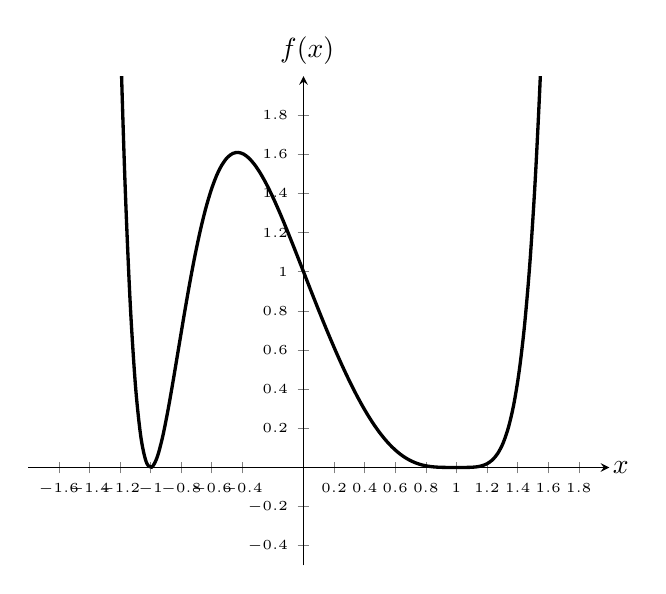
\begin{tikzpicture}
					\begin{axis}[
						scale = 0.7,
						width = \textwidth,
						every tick label/.append style={font=\tiny},
						axis x line = middle,
						axis y line = middle,
			    			every axis y label/.style={at={(ticklabel cs:1.15)}},
			    			ytick = {-.4,-.2,.2,.4,...,1.8},
							y label style={at={(axis description cs:.48,1.1)},anchor=north},
			    			ylabel = {$f(x)$},
			    			ymin = -.5, ymax = 2,
		    				every axis x label/.style= {at ={(ticklabel cs:1)}},
		    				xtick = {-1.6,-1.4,...,-.2,.2,.4,...,1.8},
		    					x label style={at={(axis description cs:1.05,.2)},anchor=east},
		    				xlabel = {$x$},
		    				xmin = -1.8, xmax = 2			
					]
						\addplot[thick, smooth, samples = 100, line width=1.2pt,domain = -1.7:1.8] {(x-1)^(4.0)*(x+1)^(2.0)*(x^2+1)};
					\end{axis}
				\end{tikzpicture}
			\end{flushleft}
		\end{ex}
			\newpage
			
		\begin{defn}[Percentage Rate of Change]
			For smooth, continuous function $f$, if the rate of change $f'(x_0)$ exists for input value $x_0$ and $f(x_0)\neq 0$, then we define the \textbf{percentage rate of change} as \showto{ins}{$\dfrac{f'(x_0)}{f(x_0)}$\\ }\showto{st}{\\[15pt] $ $ \\[15pt] $ $ \\[15pt]}
		The output for percentage rate of change is \showto{ins}{\fbox{\% per unit input}}\showto{st}{\blank{3}}.
		\end{defn}
			\vspace{.1in}
			
		\begin{ex} 
			The rate of change of the student population at OU is 2000 students per year, and the current body is 40,000 students.  Find the percent rate of change of the student population.		
		\end{ex}
			\vs{1}
			
		\begin{ex}
			For the following, use the picture:\\
			\begin{tabular}{cl}
				\begin{minipage}{.45\textwidth}
				\begin{enumerate}[(a)]
					\item At each labeled point, identify whether the instantaneous rate of change is positive, negative, or zero.
					\item Is the graph steeper at point $C$ or point $E$?
					\item Is the graph steeper at point $A$ or at point $C$?
				\end{enumerate}
				\end{minipage}
				&
				\begin{minipage}{.4\textwidth}
					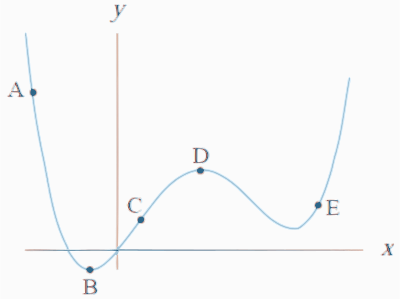
\includegraphics{./img/sec22-1.png}
				\end{minipage}
			\end{tabular}
		\end{ex}
			\vs{1}
			\newpage
			
		\begin{ex}
			The number of monthly Spotify listeners of an obscure shoegaze band is given by the function $f(x)$, where $x$ is the number of months since the release of their first album. 
			\begin{enumerate}[(a)]
				\item If the band had 3000 listeners four months after the release of their first album, and the percent rate of change was 36\% per month, find the rate of change of listeners in the fourth month to the nearest whole number.  Give a sentence of interpretation for your answer.
					\vs{1}
					
				\item A year after the release, the band had 12000 listeners.  Find the average rate of change of the band's Spotify listeners between four months and a year after the release of the first album.  Round to the nearest whole number, if necessary.  Give a sentence of interpretation for your answer.
					\vs{1}
			\end{enumerate}
		\end{ex}
			\newpage
			
		\begin{ex}
			For the following, use the picture below:\\[10pt]
			\begin{center}
				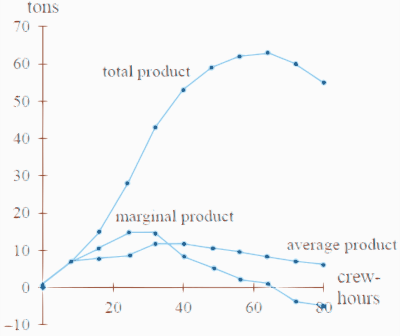
\includegraphics{img/sec22-2.png}
			\end{center}
				\vs{.1}
			\begin{multicols*}{2}
				\begin{enumerate}[(a)]
					\item For a crew working 32 crew-hours, the rate of change of which two quantities are positive?
						\vs{1}
						
					\item For a crew working 30 crew-hours, which two quantities can be improved by adding crew hours?
						\vs{1}
						
					\item At 56 crew-hours, give a relationship between the slopes of total product, average product, and marginal product.
						\vs{1}
						
					\item Starting with 24 crew-hours, which quantity has negative slope?
						\vs{1}
						\columnbreak
						
					\item The slope of which quantity is positive for less than 64 hours?
						\vs{1}
						
					\item For a crew working 75 crew-hours, the slope of which two quantities are nearly equal?
						\vs{1}
						
					\item For a crew working 24 crew-hours, which quantity is near its greatest slope?
						\vs{1}
				\end{enumerate}
			\end{multicols*}
		\end{ex}
			\newpage
			
		\begin{ex}
			For the picture below, do the following:
			\begin{enumerate}[(a)]
				\item Estimate a second point on the tangent line
				\item Calculate the rate of change of the function at the labeled point; include units and round to 2 decimal places if necessary.
				\item Calculate the percentage rate of change of the function at the labeled point; include units and round to 2 decimal places if necessary.
			\end{enumerate}
		\end{ex}
			\begin{center}
				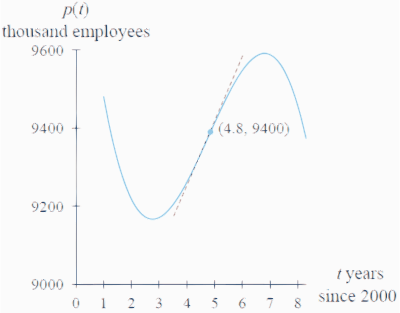
\includegraphics[scale = 1.5]{img/sec22-3.png}
			\end{center}
	\clearpage
\end{document}